\section{Grundlagen, Stand der Forschung}

\emph{Leseführung.} \lipsum[6-6]

% Und noch schnell die ganze Bibliographie zitieren:
\nocite{*}

\subsection{Theorie 1}

\emph{Informieren und orientieren.} Das Schema in Abbildung~\ref{fig:software_struktur} enthält \ldots, \lipsum[7-7]

\begin{figure}[b]
\begin{center}
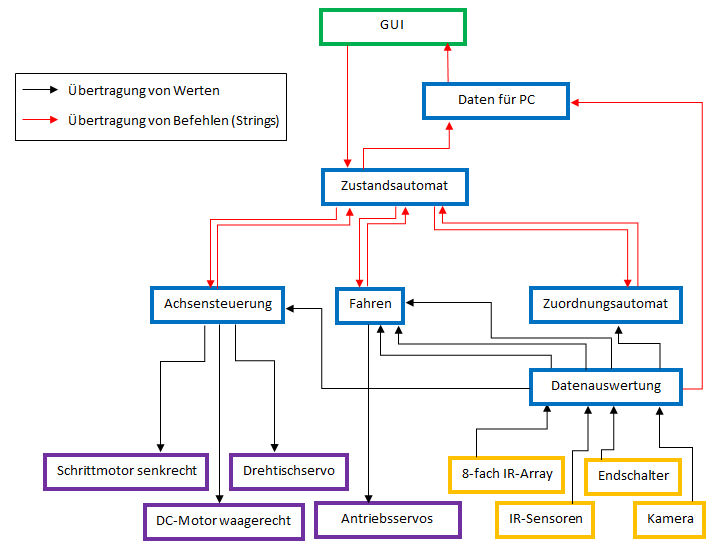
\includegraphics[width=\linewidth]{graphics/software_struktur.png}
\end{center}
\caption{Realisierte Software-Struktur in LABView}
\label{fig:software_struktur}
\end{figure}

\subsection{Unterkapitel}

\lipsum[8]  Nach Formel \eqref{eq:sincos}:
\begin{equation}
\sin \alpha \pm \sin \beta = 2\sin\frac{\alpha\pm\beta}{2}\cos\frac{\alpha\mp\beta}{2}\,. \label{eq:sincos}
\end{equation}

\lipsum[9]
\begin{equation}
x = \frac{-b\pm\sqrt{b^2-4ac}}{2a}\;.
\end{equation}

